%%%%%%%%%%%%%%%%%%%%%%%%%%%%%%%%%%%%%%%%%%%%%%%%%%%%%%%%%%%%%%%%%%%%%%%
%%%%  Load the document class and packages                         %%%%
%%%%%%%%%%%%%%%%%%%%%%%%%%%%%%%%%%%%%%%%%%%%%%%%%%%%%%%%%%%%%%%%%%%%%%%
\documentclass[a4paper]{report}
\usepackage{epsfig}            % to insert PostScript figures
\graphicspath{ 
  {./figures/} 
}

%Change figure names
\renewcommand{\figurename}{Fig}

\usepackage[bf,footnotesize]{caption} % make captions small and label bold


\addtocounter{chapter}{1} %Because starting at zero is silly
\makeatletter
\renewcommand{\thesection}{\@arabic\c@section}
\renewcommand{\thefigure}{\@arabic\c@figure}
\makeatother

\usepackage[a4paper,margin=2.7cm,tmargin=2.5cm,bmargin=2.5cm]{geometry} 
\usepackage{textcomp}          % To make nice degree symbols and others\usepackage[bf,footnotesize]{caption} % make captions small and label bold
\usepackage{wrapfig}
%to produce the clickable references along the left in Acroread. This
%package must be included last. 
\usepackage[ps2pdf,bookmarks=TRUE]{hyperref} 



%%%%%%%%%%%%%%%%%%%%%%%%%%%%%%%%%%%%%%%%%%%%%%%%%%%%%%%%%%%%%%%%%%%%%%%
%%%%  Hypertext references for Acrobat                             %%%%
%%%%%%%%%%%%%%%%%%%%%%%%%%%%%%%%%%%%%%%%%%%%%%%%%%%%%%%%%%%%%%%%%%%%%%%
\hypersetup{
pdfauthor = {SWC},
pdftitle = {Optics Exercises},
pdfkeywords = {optics, lenses, refraction, reflection, dispersion,
  telescope, microscope},
pdfcreator = {LaTeX with hyperref},
pdfproducer = {dvips + ps2pdf}
           }


\begin{document}




%set the number of sectioning levels 
\setcounter{secnumdepth}{2}

\begin{center}
\textbf{\Large{Optics Bench Exercises: Image Formation}}
\end{center}

\section{Introduction}
The goal of these exercises is to nurture an understanding of image formation, conjugate planes, and how multiple lenses interact in simple optical set ups.


\section{Before beginning}
\begin{itemize}
    \item \textbf{Do not} force parts together. All parts should screw together or fit together easily.
    \item \textbf{Do not} over-tighten screws. Gentle pressure with a long-handled Allen key is sufficient. 
    \item \textbf{Do not} touch the coated surface of mirrors or optical filters. 
    \item Each group is responsible for tidying and organising their optical set at the end of the week. All parts should be present and in their correct locations as show on the course wiki page. 

\end{itemize}

\section{Equipment usage notes}
The black post holders mount to the rail carriages via a short cap screw as shown in Fig.~\ref{fig:post}. 
The carriages can then be attached to the rail, on which they can slide up and down. 
Use the lens tool to secure lenses in lens holders. 
`SM2' refers to two inch optics and associated accessories. 
`SM1' refers to one inch optics and associated accessories. 

\begin{figure}[h]
\center
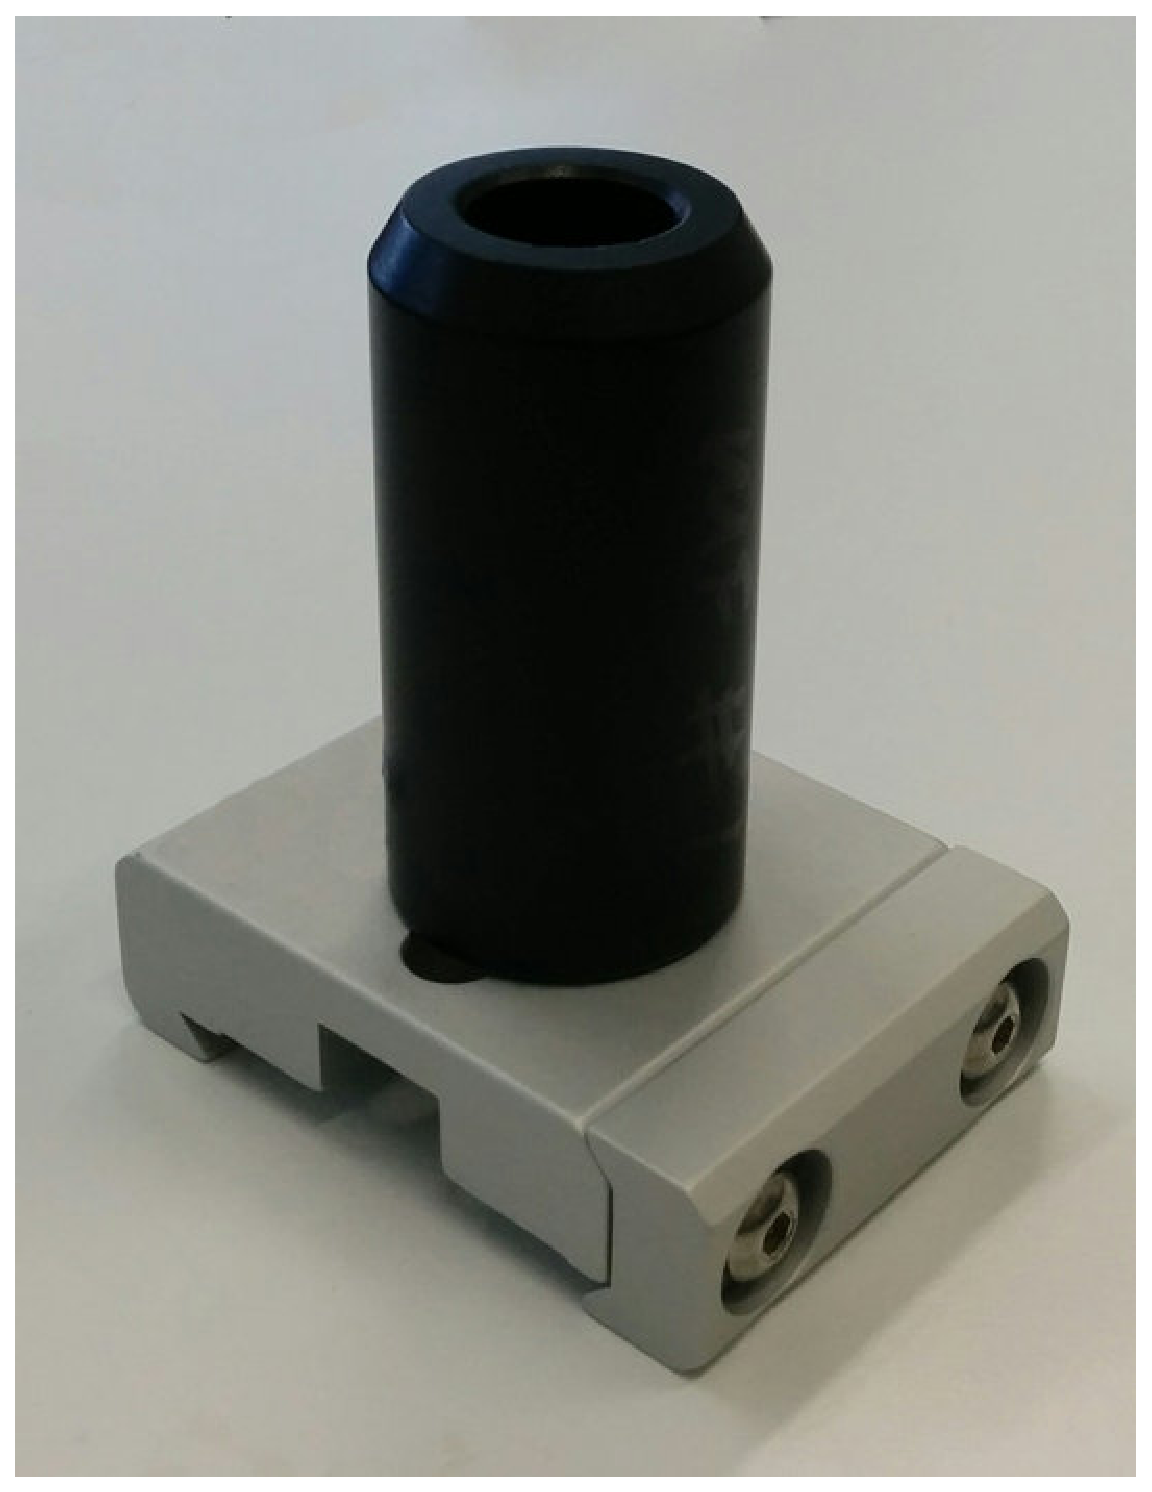
\includegraphics[width=1.3in]{post_mounted.eps}
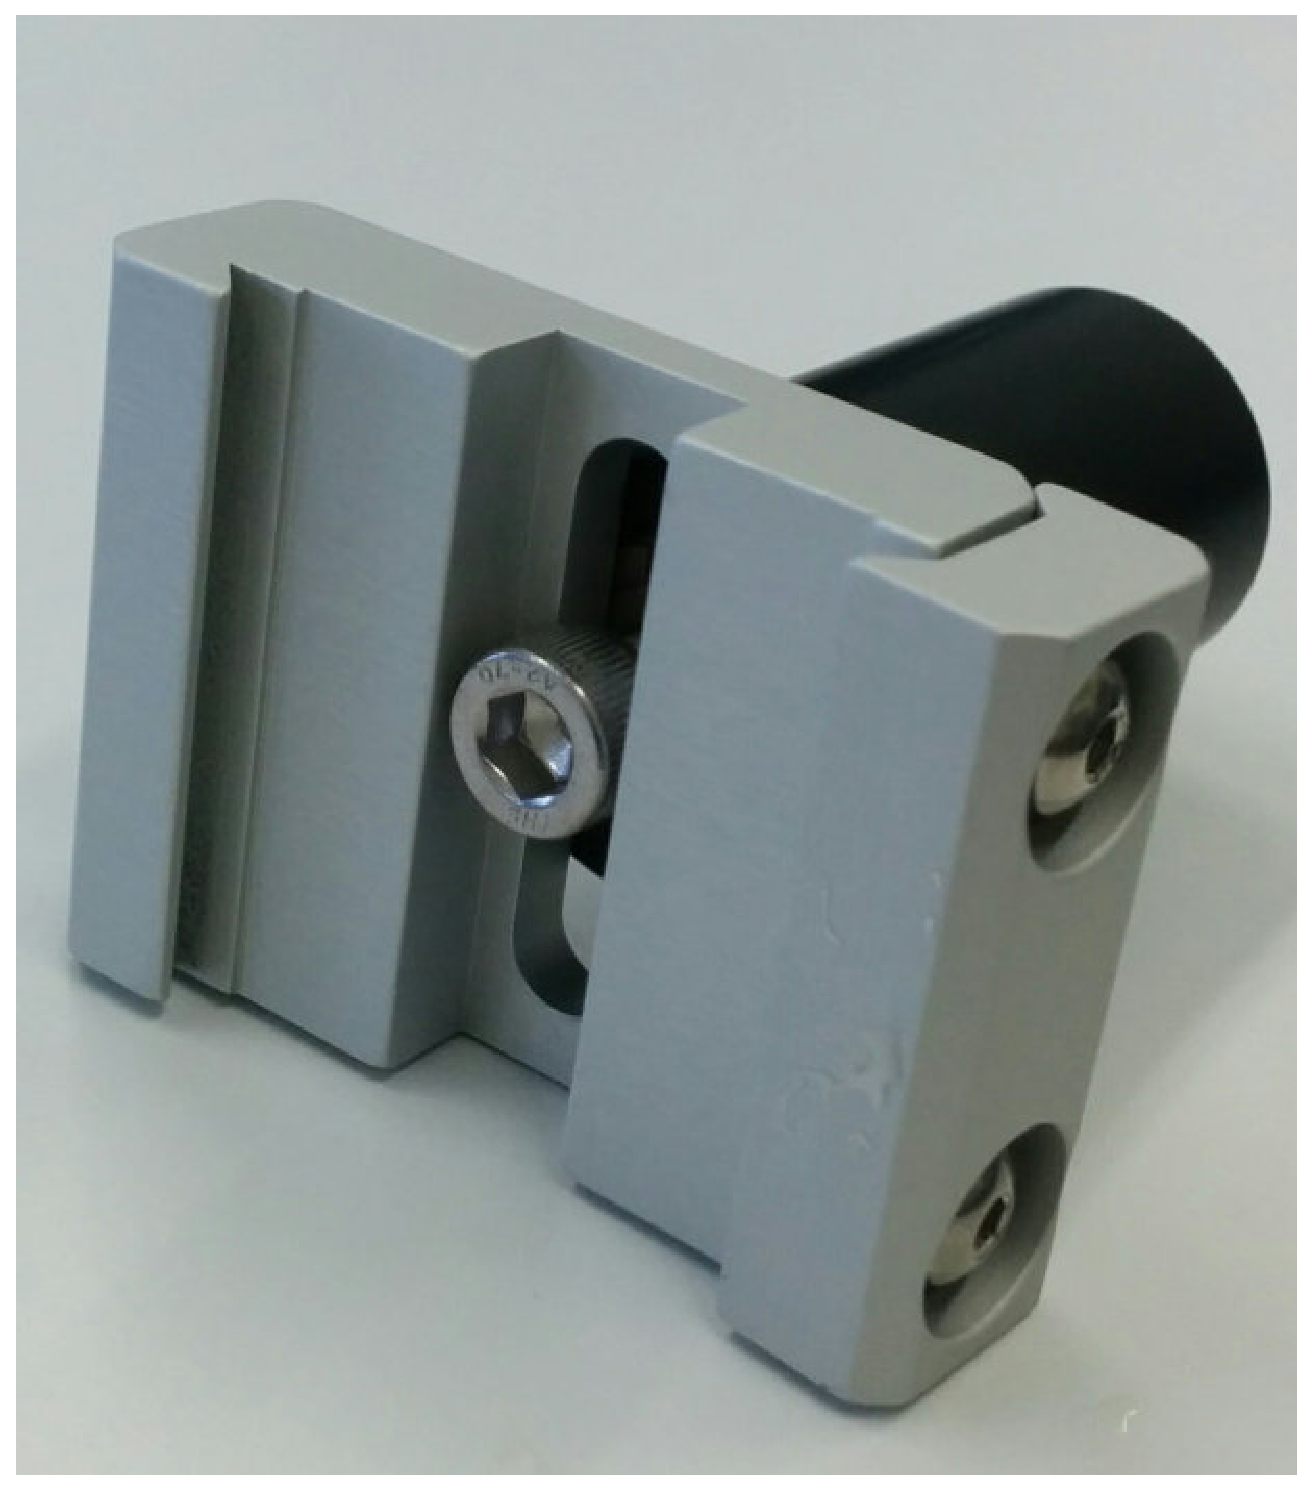
\includegraphics[width=1.5in]{post_mounted_underside.eps}
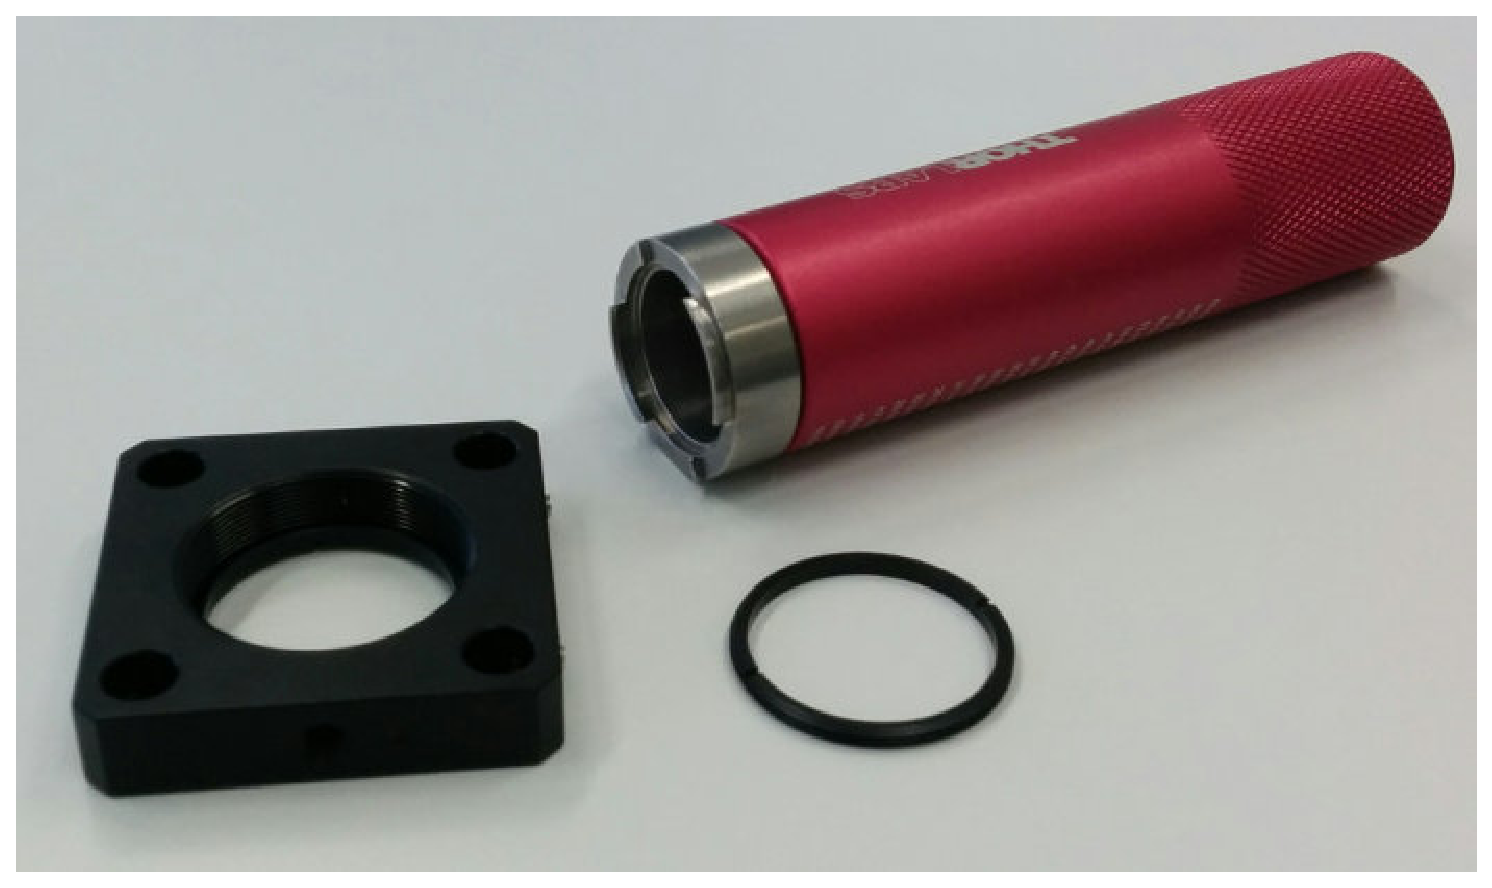
\includegraphics[width=2in]{lens_tool.eps}
\caption{A post holder bolted to a rail carriage (left \& middle).
The lens tools secure lenses in the holders using the rings (right).}
\label{fig:post}
\end{figure}


\clearpage

\section{Image Formation}
An image is formed when all light rays leaving one point (or region) of the object arrive at some other defined point (or region) \textit{regardless of the angle of the ray}. 
This is illustrated in Fig.~\ref{fig:imageforming}, where the brain cell on the left is imaged through an idealised thin lens (blue) to form the minified inverted image on the right. 
All light rays leaving the brain cell's dendrite converge onto the inverted dendrite. 
Each point in the image plane is illuminated by rays coming from a corresponding point in the object. 



\begin{figure}[h]
\center
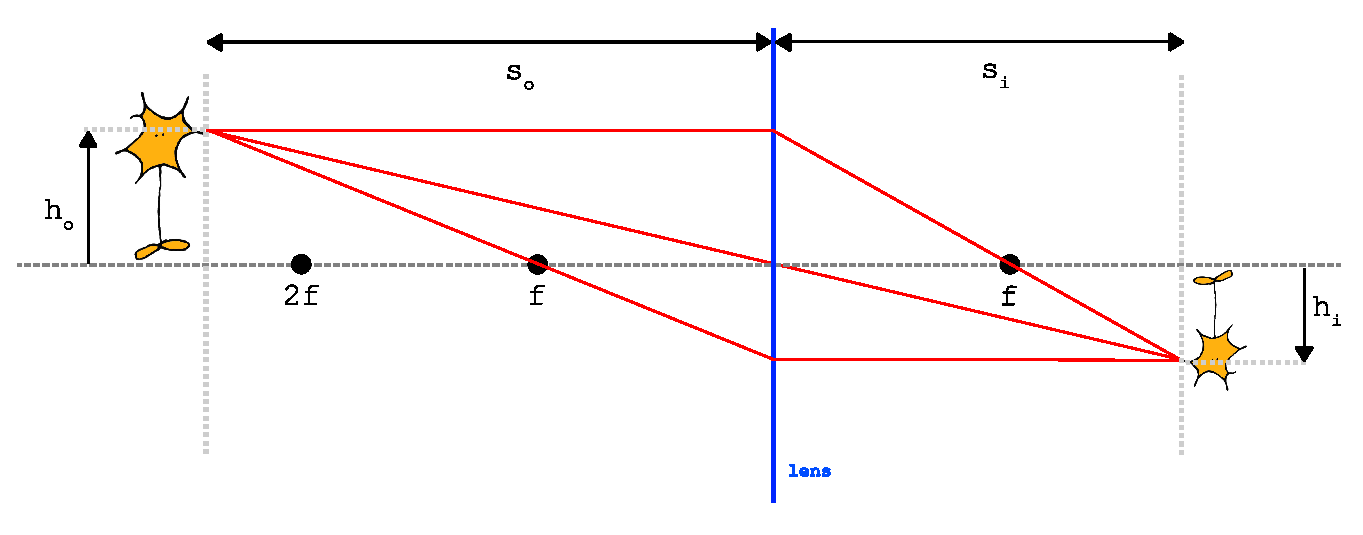
\includegraphics[width=6in]{Simple_ImageFormation.eps}
\caption{Simple image formation using one idealised thin lens (blue). 
The focal length of the thin lens is $f$, object distance is $s_o$ and image distance is $s_i$. 
The upper ray (parallel to the optical axis on the left) passes through the focal point (denoted as a dot) on the right side of the lens, the middle ray (passing through the centre of the lens) is unrefracted, and the lower ray passes through the focal point on the left side of the lens, and comes out parallel to the optical axis on the other side. 
}
\label{fig:imageforming}
\end{figure}

As the distance between the object and lens ($s_o$) is varied, the distance between the lens and image ($s_i$) also changes. This relationship is determined by the lens focal length ($f$) using the thin lens equation.

\begin{equation}
\frac{1}{s_o} + \frac{1}{s_i} = \frac{1}{f}
\label{eq:thinlens}
\end{equation}

The following conventions are used: $f>0$ for convex lenses, $f<0$ for concave lenses, $s_o$ is always $>0$, $s_i>0$ for real images, and $s_i<0$ for virtual images.
Transverse distances above the optical axis are $>0$. Distances below are negative. 

\vspace{2.5em}
You will need to get comfortable with drawing ray diagrams, since you will do this later to explain what you observe on the bench.
Copy the diagram in Fig.~\ref{fig:imageforming}.
Draw the three cardinal rays:
\begin{itemize}
\item The ray parallel to the optical axis goes through $f$ on the image side.
\item The ray that passes through the centre of the lens travels undeflected.
\item Finally, the ray that goes through $f$ on the object side leaves the lens parallel to the optical axis on the image side. 
\end{itemize}


\clearpage




\subsubsection{1. Determine the focal length of a convex lens }
For the next few exercises you will use an LED as both a light source and an object to image.
You will form various images of the LED emitter. 
Your first task is to set up the LED on the optical rail:

\begin{itemize}
\item Attach a post holder to a rail carriage (Fig.~\ref{fig:post}) and place this on the rail. 
\item Attach a 50~mm post to the white LED glued to a cage plate and place this in the post holder. 
\item Power the LED using the ThorLabs LED driver. You will need the LED power cable.
\end{itemize}


Now choose a lens with a focal length of about $f=100~mm$ and attach the lens to a lens holder using the lens wrench and a retaining ring (this should already be in the lens holder).
Mount the lens on another carriage and attach to the rail next to the LED. 
Get the LED aligned with the middle of the lens (precise alignment isn't important). 

You will use this lens to form an image of the LED.
This is called \textbf{finite conjugate} imaging because the image is paired (i.e. conjugated) with an object at a finite distance from it.
The image and sample planes are said to be \textbf{conjugate planes}.
You will be able to form an image on a piece of card or paper if the distance between the lens and LED ($s_o$) is $>1f$.
The image will be of the LED emitter, which  usually looks like a small bright square, often with fine lines going across it. 
If all you see is a blur, you have not formed an image.

\begin{itemize}
\item Place the lens $<1f$ from the LED and use a piece of card on the other side of the lens to verify that no image is formed at any distance from the lens.
\item Why is no image formed? 
Hint: draw a diagram with the object at $<1f$. Plot just two rays: the undeflected ray and the ray coming out parallel with the optical axis and then going through $1f$ on the image side. 
How do the rays behave after they have passed through the lens?

\item Verify that an image is formed when the lens is $>1f$ from the LED: place a card very far from the LED (e.g. at $10f$ or $20f$) and slowly move the lens away from the LED. 
What is the distance between the LED and the lens at which you see an image? 
It should be just over $1f$.

\item You could use the above approach to estimate the focal length of an unknown lens, however it's hard to tell when the source is at $1f$. 
What is an easier way of estimating focal length? (Hint: you may not need the rail)

\item What is the value of $s_i$ when $s_o=2f$?
\end{itemize}



\clearpage

\subsubsection{2. Magnifying the image}
As you might recall, the size of the image of the LED emitter varied with $s_o$.
A lens produces images of different magnifications depending on $s_o$; an image can always be formed when $s_o>f$. 
The magnification of a lens is calculated as follows:

\begin{equation}
M = \frac{h_i}{h_o} = -\frac{s_i}{s_o} = \frac{f}{f-s_o}
\label{eq:mag}
\end{equation}

A value of $M=1$ would mean unitary magnification (the image is the same size as the object). 
Negative numbers indicate an inverted image.

To begin thinking about magnification, hand-draw the ray diagram (as in Fig.~\ref{fig:imageforming}) for the smallest and largest values of $s_o$ that you used above. 
Make sure to give yourself plenty of room. 
Hint: You will run out of paper if you use values too close $1f$.
If you're stuck, choose $1.5f$ and $4f$.
Note the changing angles of the rays and how they lead to different image sizes as $s_o$ changes. 
We will now see what happens when the rays come from infinity:

\begin{itemize}
\item Mount a lens of about $f=60~mm$ in a holder and attach a post to it. 
Use it to form an image of the room lights on a piece of paper.
The image is formed at $1f$.
\item Repeat with a lens of about $f=100~mm$ lens. 
What two things do you notice about the image? 
\item Fig.~\ref{fig:outside} models the situation you saw. Satisfy yourself that this provides a reasonable explanation. 
\item Go back to the lens and LED.
Calculate the values of $s_o$ and $s_i$ which produce $M=-4$ (remember, negative just means inverted) for a $f=100~mm$ lens. 
Measure the size of the LED image and so calculate the size of the LED emitter. 
\item Remember the value of $s_i$ when $s_o=2f$? Therefore what is $M$ when $s_o=2f$?
\end{itemize}


\begin{figure}[h]
\center
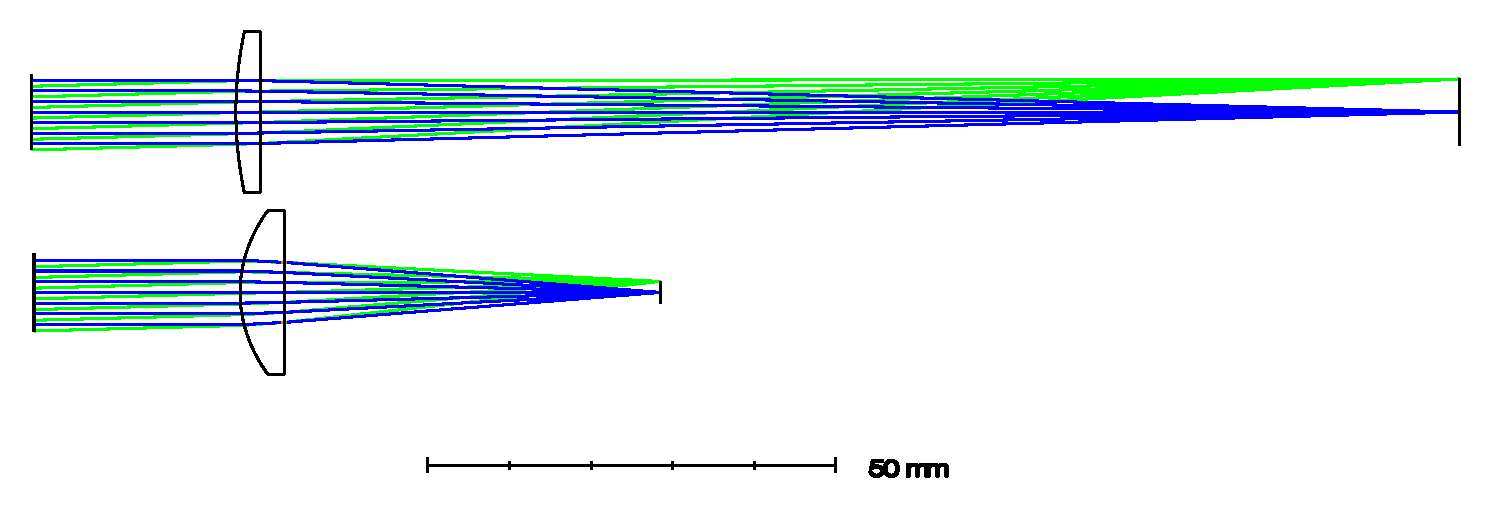
\includegraphics[width=6in]{lens_f_comparison.eps}
\caption{Images formed at $1f$ from light originating at infinity. 
The top is a $f=150~mm$ lens and the bottom a $f=50~mm$ lens.
Light from different regions of the object arrive in parallel rays that come in at different angles (green and blue). 
Each set of parallel rays come into focus at a point, satisfying the image-forming condition. }
\label{fig:outside}
\end{figure}


What you have covered above demonstrates an important property of lenses: that they work the same both forwards and backwards.
Recall the definition of an image-forming condition: \textbf{light rays leaving one point (or region) of the object arrive at some other defined point (or region)}.
This is why no image was formed when the LED was at $s_o=f$, since rays leaving the lens are parallel and do not converge on the other side. 
However, you \textit{were} able to form an image at $s_i=f$ when the object was very far away. 
The ray diagrams of these two conditions are \textit{identical}--the only difference is that the object is at $1f$ in the first case and at infinity in the second case.

\clearpage


\subsubsection{3. Virtual images}
At distances $s_o<f$, you were unable to form an image of the sample on the card because the rays emerging from the other side \textit{diverged}.
\begin{itemize}
\item Place the LED at $0.5f$ from a lens of your choice, observe the light diverging as it exits the lens.
\item Draw the ray diagram for this $0.5f$ scenario:
Draw the ray that leaves the tip of the object and continues undeflected through the middle of the lens. 
Draw the ray that travels parallel to the optical axis and goes through $1f$ on the other side.
See how these rays diverge. 
\end{itemize}

It would seem that no image is formed yet, surprisingly, a \textit{virtual image} is formed on the same side of the lens as the object. 
This may sound like a peculiar concept, but you are already familiar with virtual images as this is how you see images in flat mirrors (Fig.~\ref{fig:mirror}). 
The extended rays in the case of the mirror can be created from the \textit{diverging} rays from the object. 
In the case of the the lens at $s_o<f$ we also have diverging rays and so can also draw extended rays as we did for the mirror. 
Add the extended rays to your ray diagram by continuing the rays on the object side of the lens until they converge. 
A virtual image is formed where they converge.
What does your diagram tell you about the magnification of the virtual image?
Verify this: pick up the lens, place it $<1f$ from an object and look through it.
\begin{figure}[h]
\center
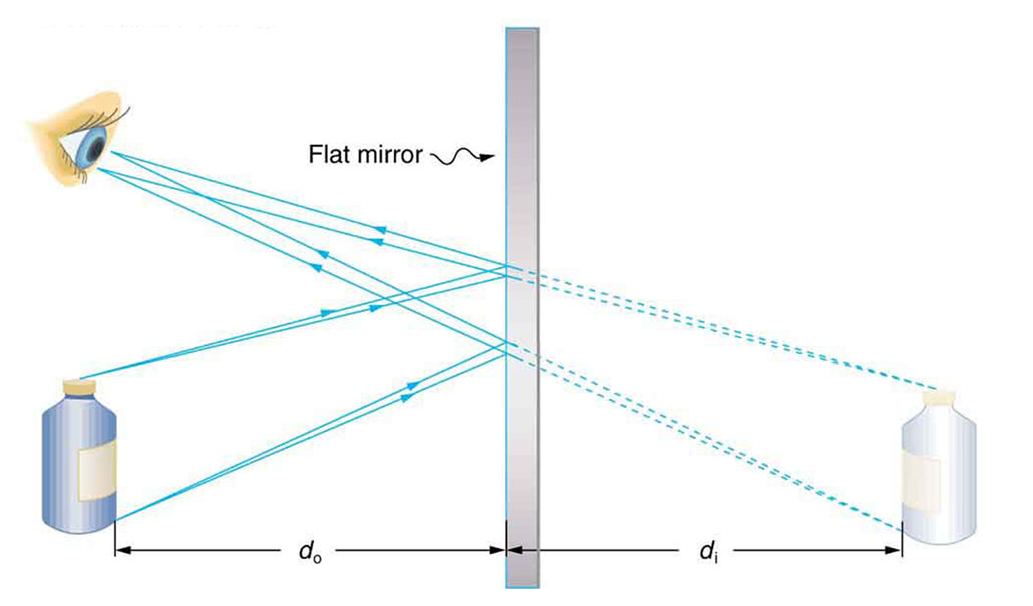
\includegraphics[width=4in]{virtual_image_mirr.eps}
\caption{A virtual image of the bottle is created on the far side of the mirror. 
This is described by the dotted lines which are `extended rays' that are used to form the virtual image. }
\label{fig:mirror}
\end{figure}

A virtual image is also formed by a negative (concanve) lens, as shown in Fig.~\ref{fig:neglens}. 
Examine the ray diagram of the negative lens. 
What do you predict you will see if you look through a negative lens?
Verify this with the $f=-50~mm$ lens.
\begin{figure}[h]
\center
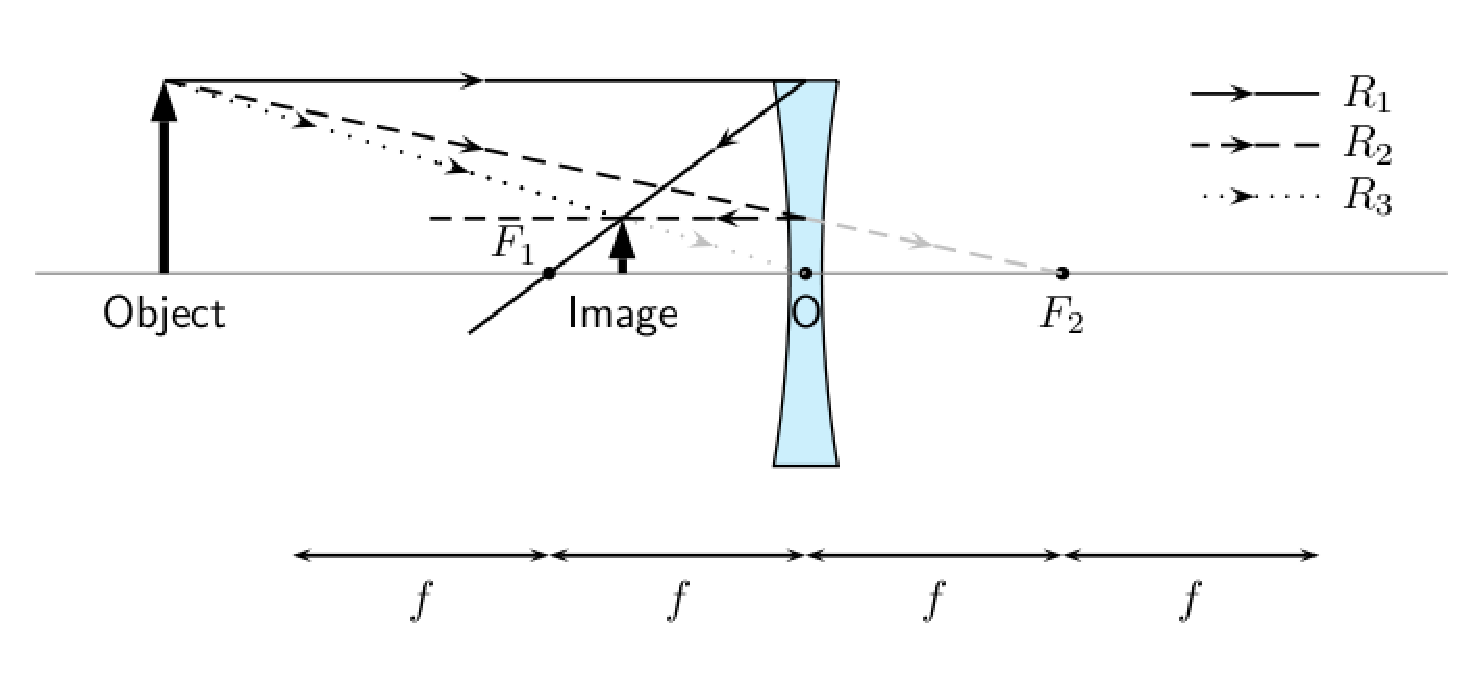
\includegraphics[width=3.5in]{negative_lens.eps}
\caption{Ray diagram of a negative lens.}
\label{fig:neglens}
\end{figure}

In summary, a \textbf{real image} is formed on the opposite side of the lens to the sample. 
This allows the detector to be physically separated from the sample, which is rather useful.
A \textbf{virtual image} is formed on the \textit{same} side of the lens as the object. 

\clearpage

\subsection{Infinite Conjugate}
The \textbf{infinite conjugate} refers to the situation where the object is located at a distance of $1f$ from a lens (Fig.~\ref{infiniteConjugate}). 
In this scenario the rays leaving the lens are parallel and do not converge, so this is not an image forming condition. 
Instead, the image can be considered to be infinitely far away (hence the name). 
If a second lens is added, then an image can be formed. 
The magnification of the image is defined as Eq.~\ref{eq:magIC}. 
This arrangement is useful because the image is always formed at $1f$ from the second lens irrespective of the distance between the lenses.
Most microscope objectives are designed to work in this configuration since it allows filters to be added into the infinite space without altering the location of the image plane. 
Such objectives are known as `infinity corrected', since they are designed to produce their best images with the sample at $1f$.

\begin{equation}
M=-\frac{f_2}{f_1}
\label{eq:magIC}
\end{equation}

\begin{figure}[h]
\center
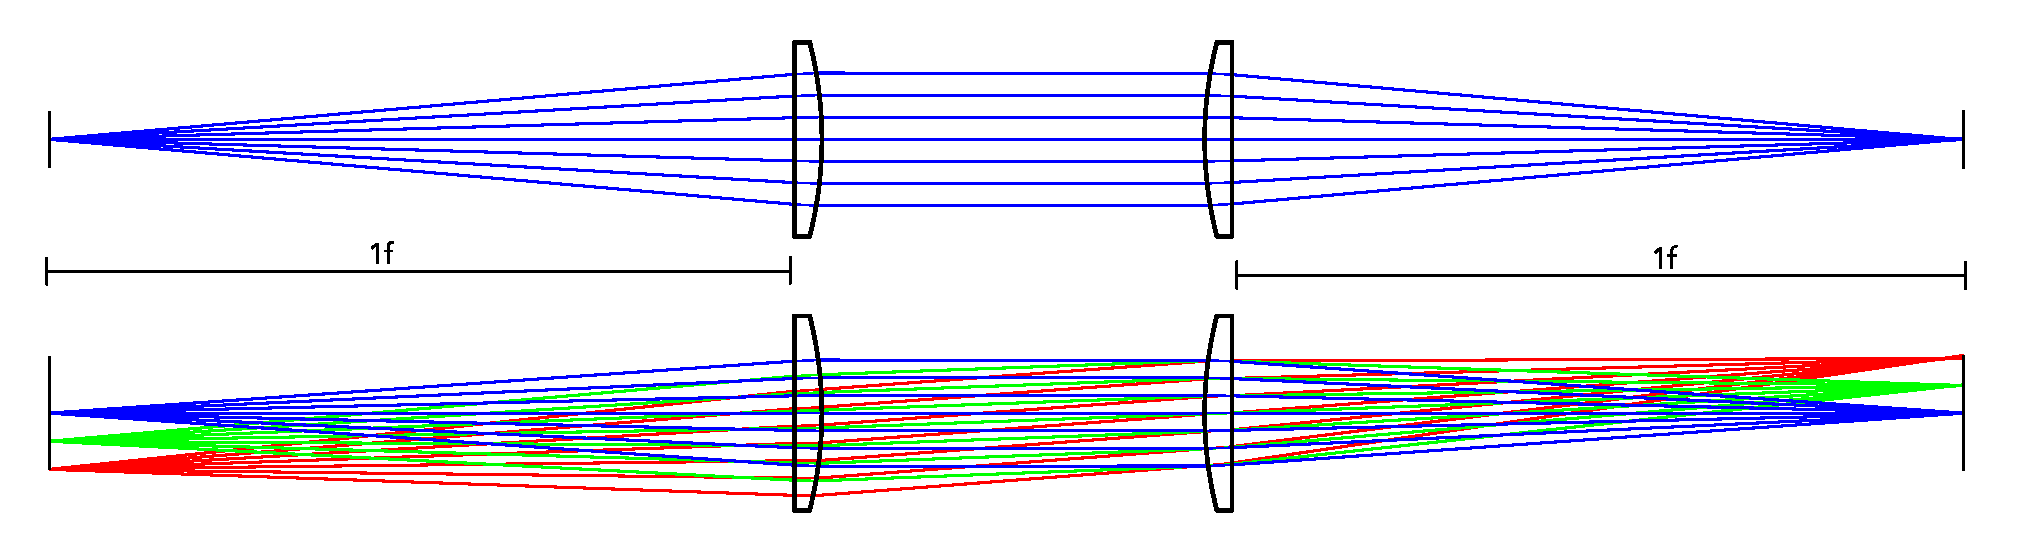
\includegraphics[width=6in]{Inf_Conf_100mm.eps}
\caption{Two views of an infinite conjugate system made up of two $f=100~mm$ lenses. 
The upper image shows on-axis rays only. 
Note the rays are parallel in the infinite space.
The lower diagram shows two additional sets of rays which arise from different off-axis locations and converge into corresponding locations in the image plane. }
\label{infiniteConjugate}
\end{figure}

\begin{itemize}
\item Set up two lenses with different focal lengths on the rail to build the infinite conjugate. 
Ensure that the first lens is at $1f$ from the LED before placing the second lens. 
\item Place a screen at the $f$ of the second and hold it in place with the post-mounted clip.
\item Verify the consequences of the infinite space by moving the second lens and maintaining the screen at $f$ of the second lens. 
What happens to the image size?
\item Swap the first lens with one of a different focal length. 
Verify that the image size changes in the manner in which you expect. 
\end{itemize}



\clearpage


\subsection{Beam expanders}
Lenses can be used to expand the diameter of a light beam, such a laser.
Expanders can be built using either two convex lenses (Fig.~\ref{beamExpander1}) or a convex and concave lens (Fig.~\ref{beamExpander2}). 
In both cases the lenses are set up such that their focal points coincide (i.e. they are separated by the sum of their focal lengths). 
The image formed by the first lens is imaged at infinity by the second lens.
The degree to which a beam is expanded is given by:
\begin{equation}
\frac{d_2}{d_1}=\frac{f_2}{f_1}
\label{eq:beamExp}
\end{equation}

\begin{figure}[h]
\center
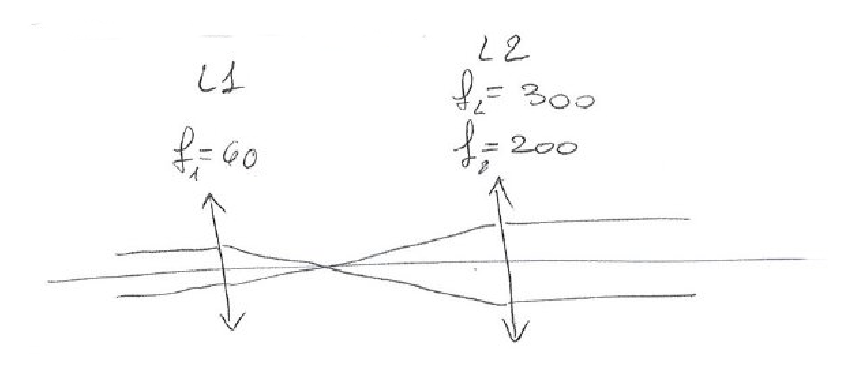
\includegraphics[width=4.5in]{beamExpander1.eps}
\caption{Beam expander with two convex lenses.}
\label{beamExpander1}
\end{figure}

\begin{figure}[h]
\center
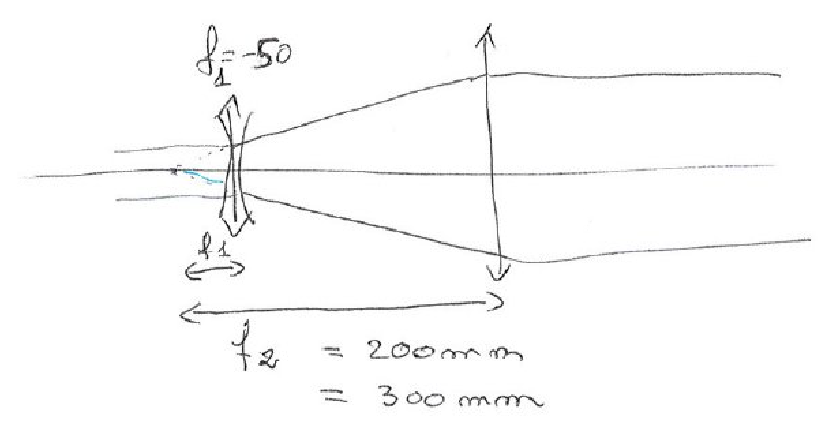
\includegraphics[width=4.5in]{beamExpander2.eps}
\caption{Beam expander with one convex and one concave lens.}
\label{beamExpander2}
\end{figure}

We need collimated light (parallel rays) entering the system, so swap the LED for a laser pointer.
You will clamp your laser pointer and align it to the rail (i.e. have the beam traveling parallel with the rail). 
The lenses will then be aligned with respect to the beam. 
This is an easy way of producing a well-aligned optical system and you will use it again later in the practical.
The procedure is as follows:

\begin{itemize}
\item Attach an RA180 clamp to a 75 mm post (the irises are mounted on 75 mm posts) and clamp the laser pointer to it (Fig.~\ref{fig:mounted_laser}).
\item Place the pointer at one end of the rail.
\item Place the iris next to the laser pointer, close it and adjust the height of the laser pointer so the beam goes through the hole. 
\item Slide the iris to the other end of the rail. 
\item \textit{Rotate} the post the laser pointer sits on and change the clamping force to \textit{tilt} the pointer until the beam goes through the iris. 
\textbf{Do not translate the laser pointer up and down.}
\item Slide the pointer back down the rail and confirm that the beam still passes through hole. 
If not, \textit{translate} the laser pointer's post up and down, then repeat the previous step.
\end{itemize}

\begin{figure}[h]
\center
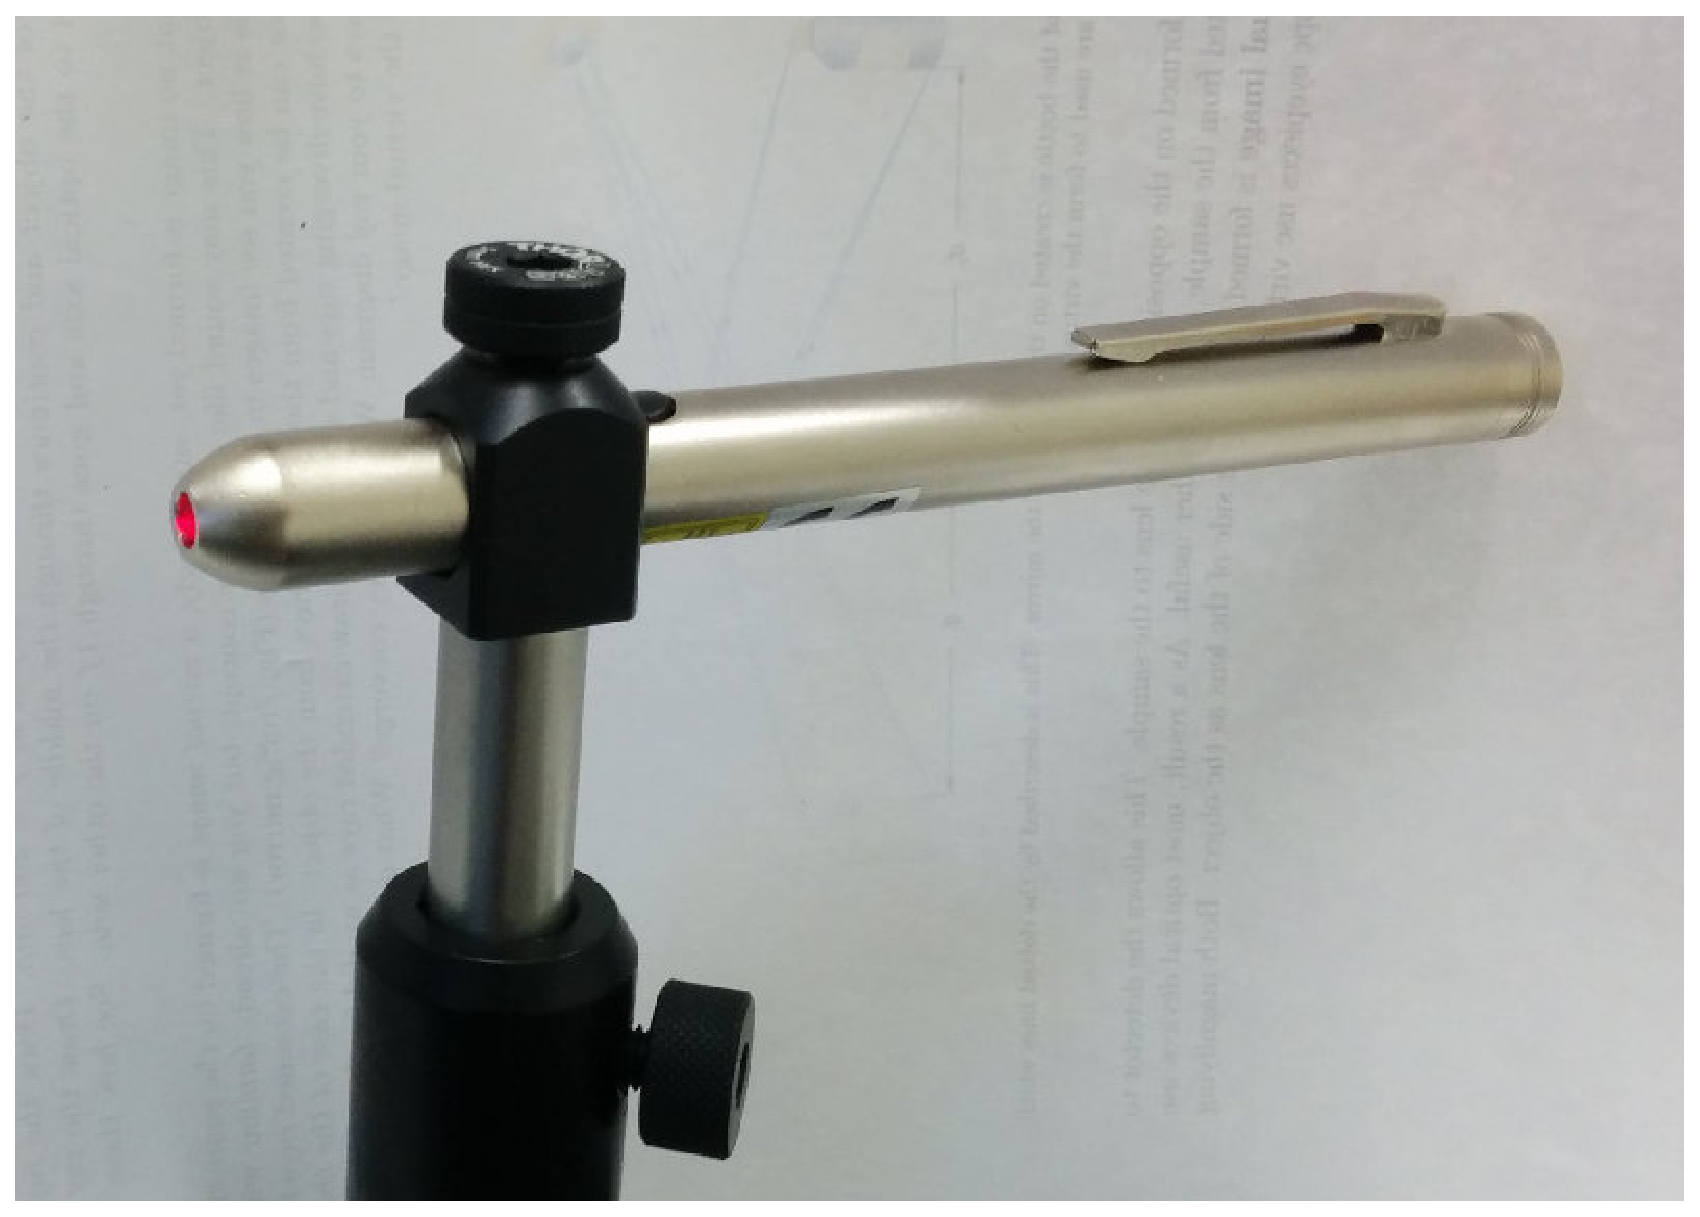
\includegraphics[width=3in]{mounted_laser.eps}
\caption{Laser mounted on a post.}
\label{fig:mounted_laser}
\end{figure}


Now you will build a 3x beam expander $f=300~mm$ lens and an $f=100~mm$ lens. 
These will be placed at the sum of their focal lengths and the laser pointer will be used as a guide for placing the lenses. 

\begin{itemize}
\item Place two more rail carriages onto the rail, between the iris and the laser pointer. 
\item Place the $f=100~mm$ lens onto the post carriage nearest the laser and position the iris roughly $1f$ from the lens.
\item You will know the lens is at the correct height because the beam will hit the middle of the iris. 
If you look carefully at the lens surface, you can also judge the height by looking at the back-reflection of the beam on lens surface. 
\item Slide the iris down the rail and complete the expander with the $f=300~mm$ lens. Again, use the iris as a target to judge lens height.
\item Make sure that the two focal points coincide by checking that the exit beam remains collimated (does not diverge or converge)
at all distances from the second lens. 
\item Measure the size of the expanded beam and so calculate size of the unexpanded beam.
\item Swap out the $f=100~mm$ lens with the $f=-50~mm$ concave lens. Verify that the expanded beam diameter doubles. 
What advantages does the negative lens add?
\item Build a beam expander to yield the maximum magnification your optics kit allows (e.g. $f=300~mm$ and $f=30~mm$ to yield 10x). 
The beam expander you have built also goes by another common name.  What is it? 
Hint: think about what happens to beams that do not travel on-axis (Fig.~\ref{fig:telescope}).
Once you've figured it out, remove the laser pointer and use your device. 
\end{itemize}


\begin{figure}[h]
\center
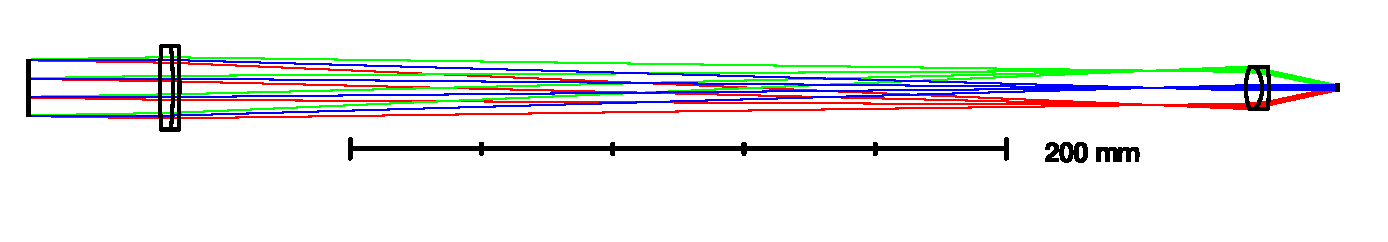
\includegraphics[width=6in]{Telescope.eps}
%\includegraphics[width=3in]{Telescope_Obj.eps}
%\includegraphics[width=3in]{TelescopeEyepiece.eps}
\caption{A beam expander composed of an $f=300~mm$ lens and an $f=25~mm$ lens. 
In addition to the collimated beam arriving on-axis (blue), two off-axis beams are shown in different colors.
Note how the angles of the beams leaving the $f=25~mm$ are substantially larger.}
\label{fig:telescope}
\end{figure}

\clearpage


\subsection{Optics Challenge}
Arrange 4 lenses, one of which must be a negative lens, so as to form a de-magnified, real, upright image. Hints: 
\begin{itemize}
\item Space will be a problem: the lenses will take up the whole rail and so you will need to place the target and screen outside of the rail.
\item Use a bright light source to illuminate your target or the image will likely be dim. 
\item There are multiple solutions to this problem.
\end{itemize}




\subsection{Bonus Exercise: Compound Lenses \& Optical Aberrations}
\begin{wrapfigure}{R}{0.22\textwidth}
  \begin{center}
    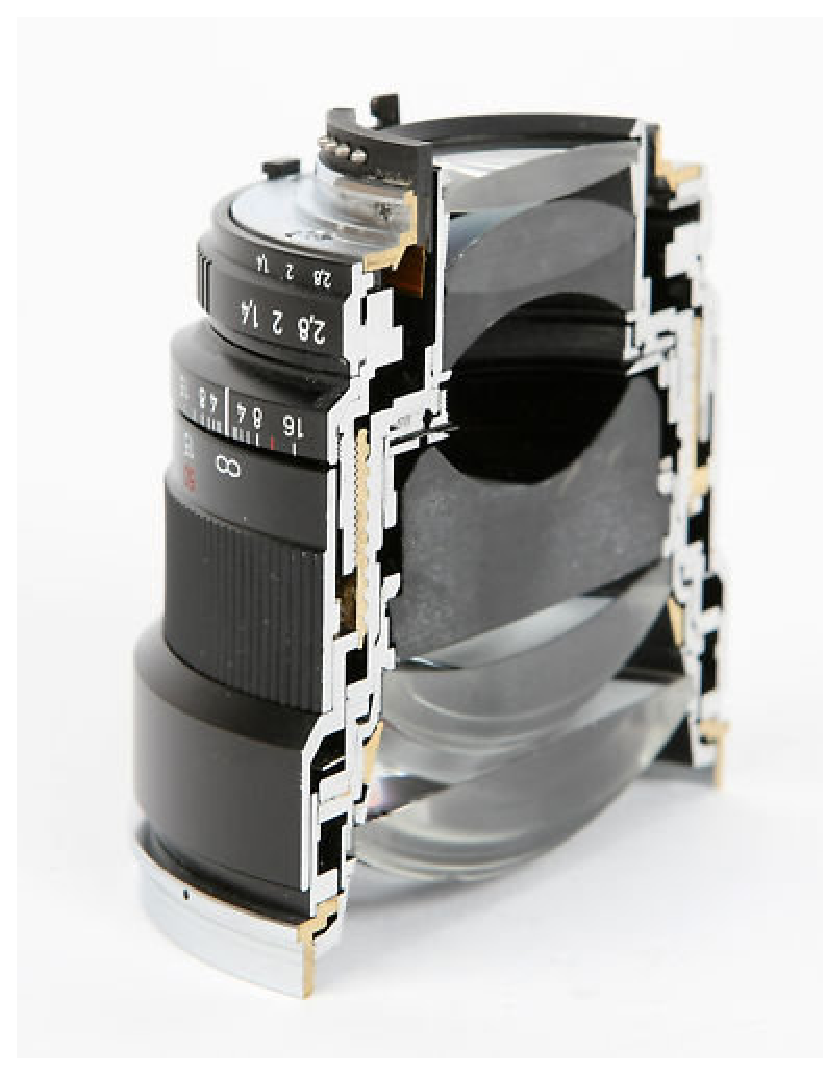
\includegraphics[width=0.22\textwidth]{SLR_lens_cut_in_half.eps}

  \end{center}
  \vspace{-100pt} 
\end{wrapfigure}
In this optional exercise you'll explore image aberrations and see why camera lenses, microscope objectives, and eyepieces contain multiple lenses spaced closely together. 
You will do this by building a variety of simple telescopes and assessing their image quality.
After this exercise you will have learned:
\begin{itemize}
    \setlength\itemsep{0.15em}
    \item Why thin lens ray tracing does not capture aberrations.
    \item What is chromatic aberration and how it can be corrected.
    \item What are spherical aberration (SA) and coma.
    \item How aberrations can be reduced by using smaller ray angles.
\end{itemize}


\subsubsection{Limitations of the thin lens approximation}
The ray tracing you've learned is good for planning simple optical systems but offers no information about image quality. 
This is because your ideal `thin lenses' always observe the image forming condition: all rays leaving a point on the sample plane converge onto a point on the image plane. 
In reality the image forming condition does not always hold. 
Rays hitting the lens at steeper angles will come into focus at a position other than that predicted by thin lens ray tracing. 
This is worse for steeper ray angles and more curved lenses. 
Image `\textbf{aberrations}' occur when rays leaving a point in the sample do not all converge in the image plane.
Rays instead converge in different locations according to a systematic pattern which depends upon the form of the aberration. 
The the three most common aberrations are chromatic aberration, spherical aberration, and coma (Fig.~\ref{fig:aberrations}). 

\begin{figure}[h]
\center
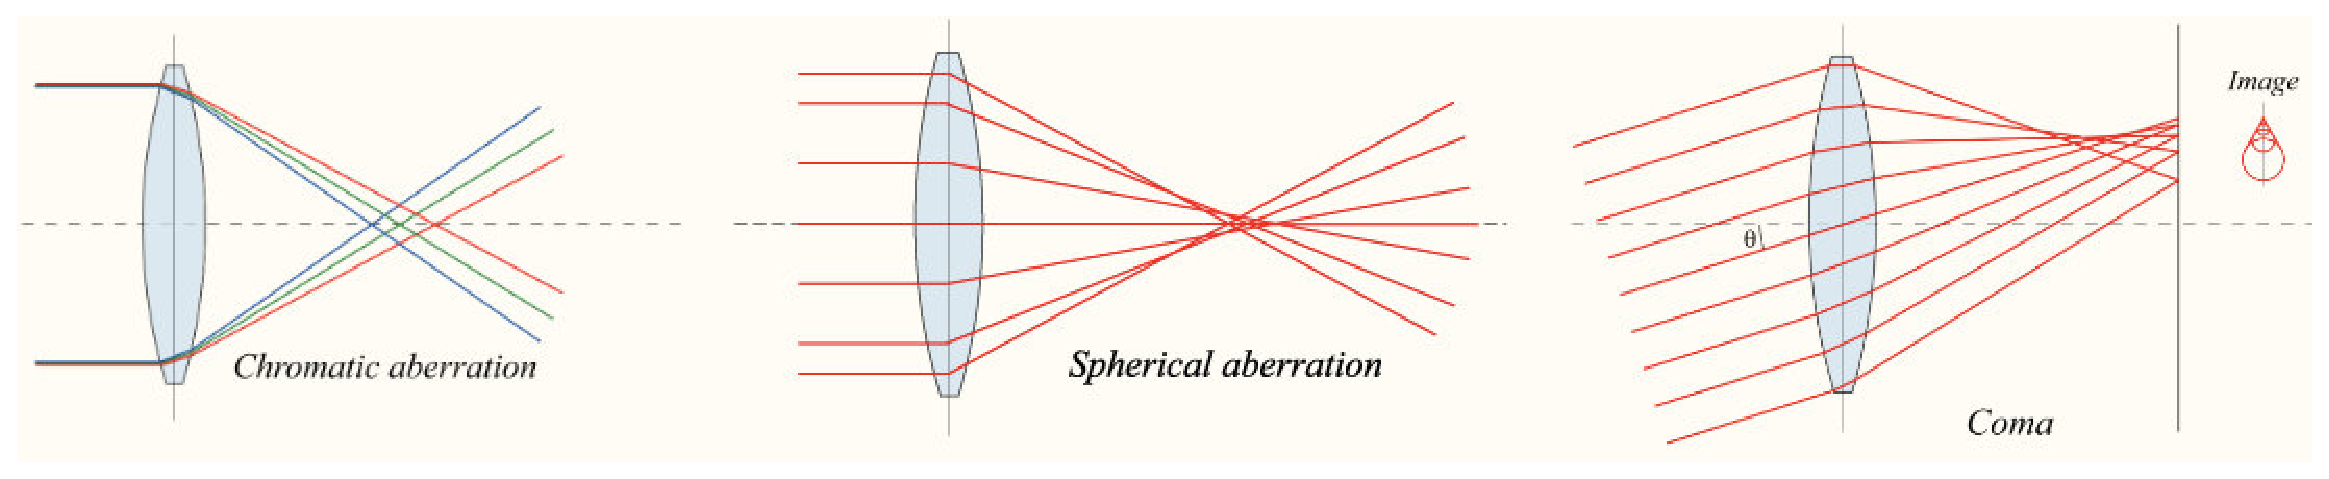
\includegraphics[width=6in]{aberrations.eps}
\caption{ 
Chromatic aberration sees light of different wavelengths coming into focus at different distances from the lens.
Spherical aberration sees on-axis light (that parallel to the optical axis) having different focal lengths depending upon distance from the optical axis. 
Coma is the situation where off-axis light does not come into focus in the same spot. Coma does not occur for rays traveling along the optical axis.}
\label{fig:aberrations}
\end{figure}



\subsubsection{Chromatic aberration}
Blue light is refracted more strongly than red light and so the focal length of a lens is wavelength dependent. 
Lenses therefore have shorter focal lengths for blue light than red light (Fig.~\ref{fig:aberrations}).
This leads to a pronounced wavelength-dependent blurring of the image known as chromatic aberration. 
You will now build a telescope on the 500 mm optical rail:
\begin{itemize}
\item Use an f=300~mm for the objective and an f=25~mm for the eyepiece. 
\item Look through your telescope at an object across the room. How does the chromatic aberration manifest itself?
\item Ask for the f=300~mm achromat and swap your singlet lens with this. Observe the image again.
\end{itemize}

\textbf{How does it work?} 
The first element of the achromat is a positive lens that will converge light. 
The second element is a negative lens that will diverge light.
This second element has a lower power and so together the elements of the achromat constitute a positive lens. 
The two elements are made of glass with different indexes of refraction. 
The second (negative) element has a stronger index of refraction. 
Thus, the second lens diverges blue light more strongly than the first lens can focus it.
This balancing act is finely tuned to bring red and blue light into focus at the same spot.

Coarsely speaking, the second lens of the achromatic doublet disperses light in the \textit{opposite direction} to the first lens in order to bring different wavelengths into a common focus. 
\textbf{Aberrations are generally corrected by adding an element which introduces the opposite aberration.}






\subsubsection{Spherical Aberration \& Coma and Ray Angles}
Look through your telescope and pay attention to how the image quality varies across the field of view. 
What do you see?
What you see is likely due to various different aberrations. 
Let's try to clean up the image. 

Examine Fig.~\ref{fig:aberrations}, whilst it doesn't show how SA and coma arise it does allow us to predict that these aberrations will be less prominent if the outer rays are removed. 
Place an iris on a rail carriage and locate it around 15 cm behind the objective lens. 
Close the iris whilst looking through the telescope. 
As the iris closes, fine features at the edges of the field will become sharper but the field of view doesn't change. 




\subsubsection{Compound Eyepieces}
Using an iris (known as a `pupil') to reduce ray angles is a common approach for taming aberrations but it is limited since it of course also reduces light. 
A better approach is to choose lenses such that you avoid introducing aberrations in the first place. 
You will now replace the $f=25~mm$ lens with a compound lens of similar focal length (Eq.~\ref{eq:compoundLensF} shows how to calculate the effective focal length of two thin lenses separated in air by some distance $d$). 
A compound lens is one where the optical elements are spaced closely together. 
Ask for one of the two compound lenses: one is is composed of two plano-convex singlet lenses (Fig.~\ref{fig:composite}, right)
and the other is known as a Pl\"{o}ssl eyepiece, which is composed of two closely spaced achromats. 
In what ways has the image improved compared to the single $f=25~mm$ lens?
Is the Pl\"{o}ssl better than the singlet pair?

\begin{equation}
\frac{1}{f} = \frac{1}{f_1} + \frac{1}{f_2} - \frac{d}{f_1f_2}
\label{eq:compoundLensF}
\end{equation}


\begin{figure}[h]
\center
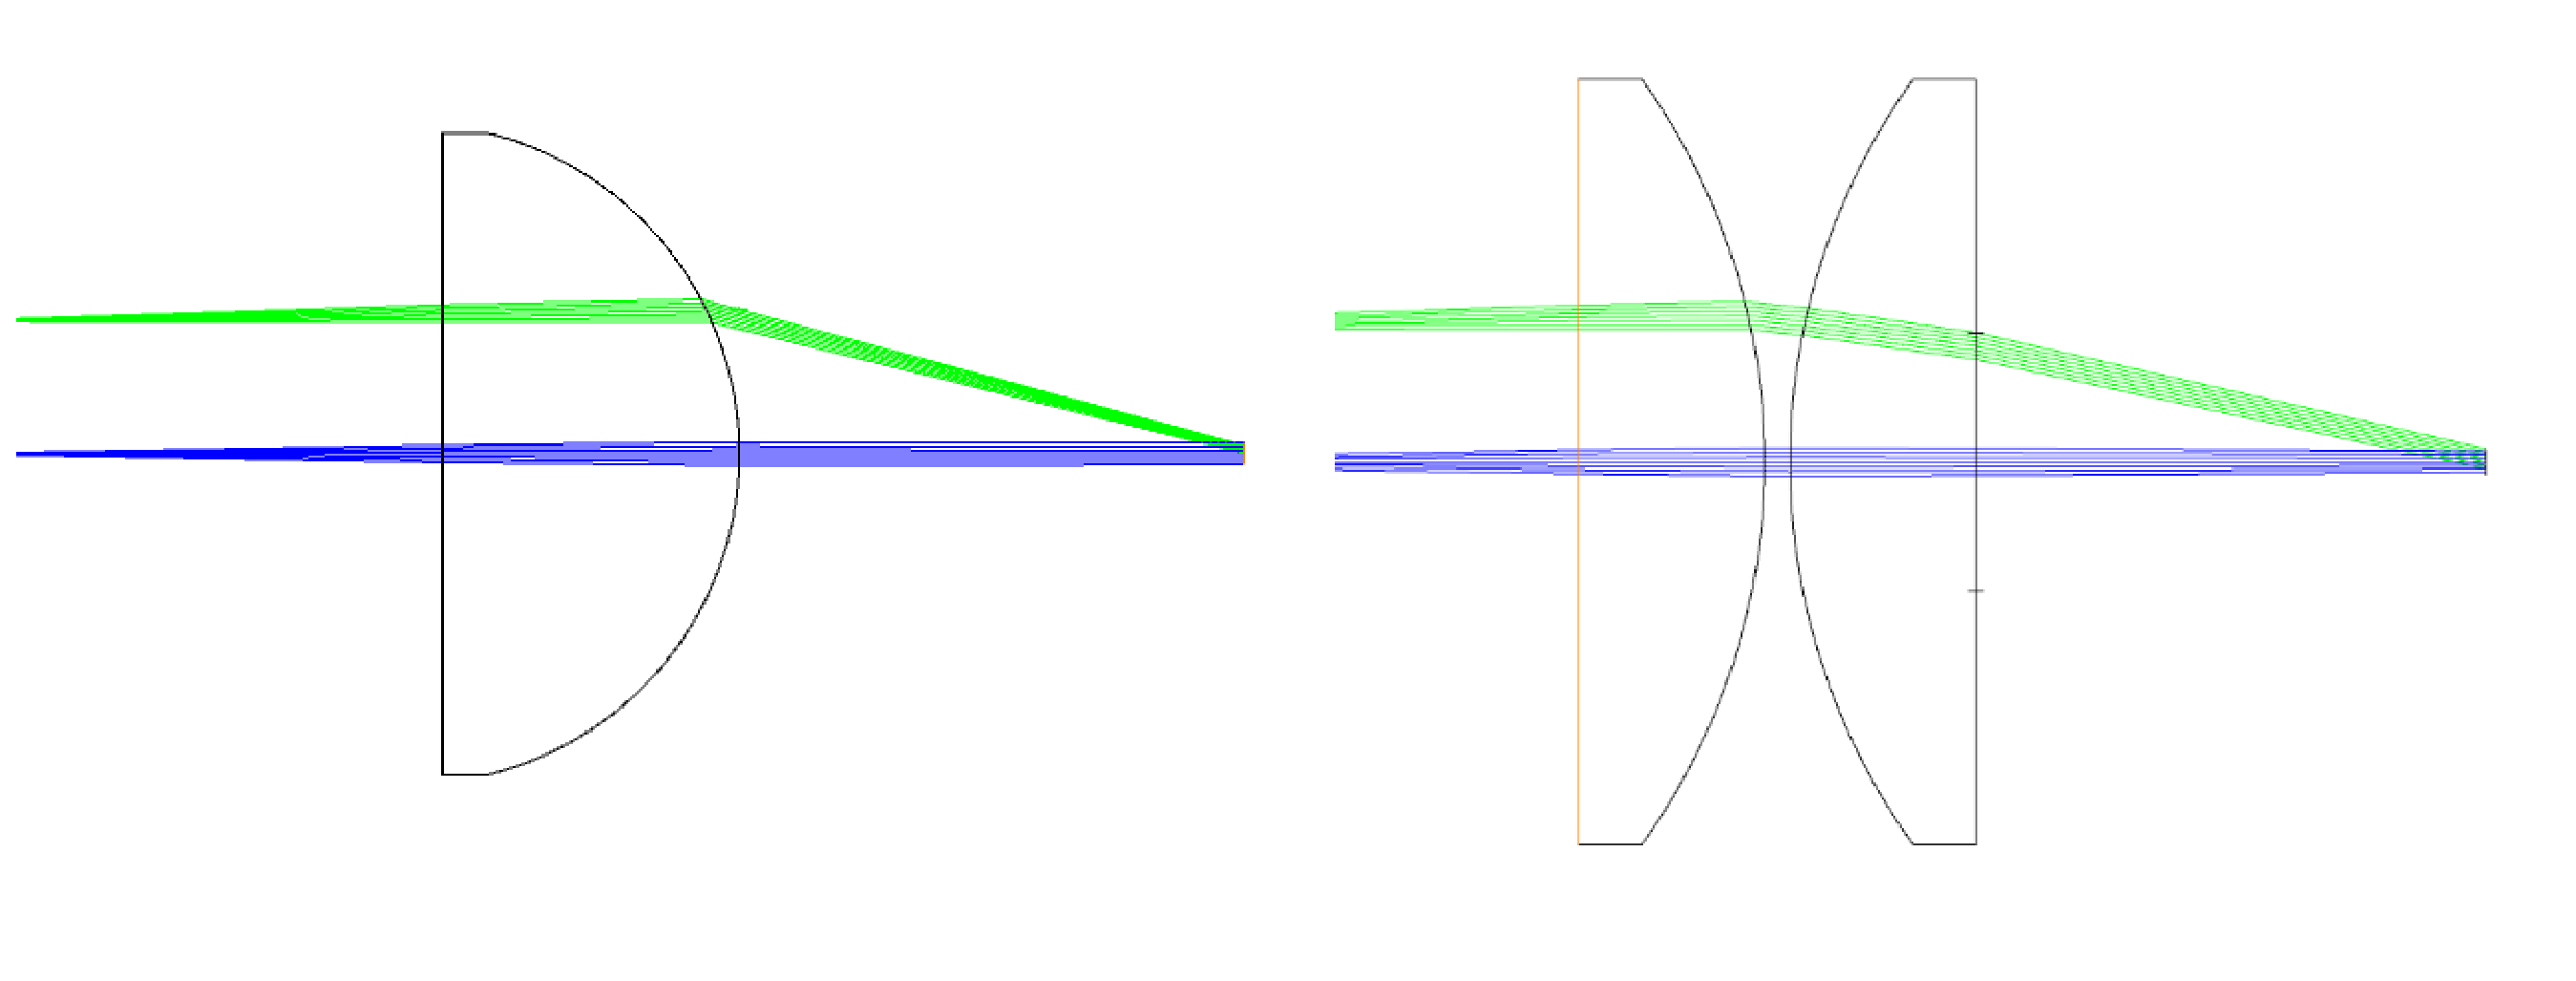
\includegraphics[width=4.5in]{eyepiece_compare.eps}
%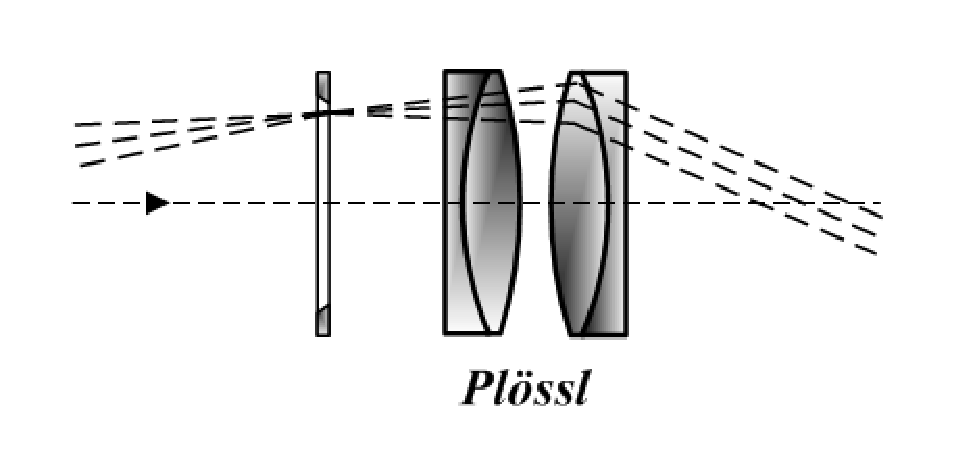
\includegraphics[width=2.15in]{Plossl.eps}
\caption{Ray diagrams of two of the eyepieces you have access to. Left: $f=25~mm$ plano-convex singlet (you might have a bi-convex version). 
Right: $f=25~mm$ compound lens composed of two $f=50~mm$ singlet lenses. 
Blue rays are on-axis. 
Green rays arise from an object 1 degree off-axis. }
\label{fig:composite}
\end{figure}


\textbf{Why does the compound lens clean up the image edges?} 
The simple answer is that the singlet lens must bend off-axis light by a large amount as it exits (Fig.~\ref{fig:composite}) and this is sufficient to induce large aberrations. 
Even in this low resolution ray diagram, you can see that the green ray is not collimated upon exiting the lens.
The doublet lens spreads the `work' across more surfaces and so avoids introducing aberrations. 
The green rays leaving the final surface remain collimated. 



\end{document}
